\section{Research Idea 5: Explicit Geometry and Human Pose for Social-Norm Reasoning}
\subsection{Initial Implementation}
\label{sec:idea5-impl}

\paragraph{Task and inputs.}
EgoNormia asks for the normatively appropriate next action in an egocentric clip and its justification, each from five options plus ``None of these'' (never gold on our test set). We report \emph{joint accuracy} (both heads correct) on the 200 verified items $T$; training and cross-validation use 600 further items from disjoint source videos. Each item is a strip of five pre-action RGB frames, the same frames rendered as depth (Depth-Anything-V2-Small), instance-segmentation (YOLOv8n-seg) and body/hand-skeleton (MediaPipe) maps, and one spatial description per image written by Gemini~4 without seeing the question. The same extractors yield four spatial labels per item (people count, nearest-person distance, facing, hands visible).

\paragraph{Controls.}
Every spatial arm has a matched control with the same amount of non-spatial content: maps and descriptions from another item (\emph{mismatched}), the RGB strip repeated, EgoNormia's own non-spatial scene description, or, for training, an identical LoRA on non-spatial data. A \emph{spatial-specific} effect is a spatial arm minus its matched control; a gain over RGB alone does not show spatial transfer.

\paragraph{Universal embedding.}
A frozen Qwen3-VL-Embedding-8B encodes the context as one L2-normalised vector $\mathbf c$ and each option as $\mathbf o$. Conditions are C2 (RGB plus its description), C5 (C2 followed by each map and its description; our combined embedding), X1 (C5 with another item's maps and descriptions) and X3 (C2 with the strip repeated). A low-rank bilinear scorer with an option prior and an abstention bias,
\begin{equation}
s(\mathbf c,\mathbf o)=\alpha\,\mathbf c^{\top}\mathbf o+(A\mathbf c)^{\top}(B\mathbf o)+\mathbf v^{\top}\mathbf o+\beta\,\mathbf 1[o=\text{None}],
\end{equation}
is trained with softmax cross-entropy over the options $O^{h}_i$ of each head $h\in\{a,j\}$,
\begin{equation}
\begin{split}
\mathcal L_{\mathrm{sc}}={}&-\tfrac1N\textstyle\sum_{i}\sum_{h}\log p\big(y^{h}_i\mid\mathbf c_i,O^{h}_i\big)\\
&+\lambda\big(\|A\|_F^2+\|B\|_F^2+\|\mathbf v\|^2\big),
\end{split}
\end{equation}
and evaluated by 5-fold cross-validation grouped by source video (800 items) and on $T$. A logistic probe on $\mathbf c$ reads out the spatial labels (balanced accuracy); as the labels share extractors with the maps, it is only a manipulation check.

\paragraph{Direct answering.}
Gemini~4, GPT-5.6 and Qwen3-VL-32B answer from RGB alone and with maps, mismatched maps, RGB repeated or descriptions; from text-only descriptions (reworded vs.\ \emph{spatially reversed}, every left/right, near/far and toward/away flipped); with spatial vs.\ generic chain-of-thought; and under forced choice with ``None'' removed.

\paragraph{Spatial fine-tuning.}
Qwen3-VL-8B is LoRA-tuned ($r{=}16$) with $\mathcal L_{\mathrm{SFT}}=-\sum_{t\in\mathrm{ans}}\log\pi_\theta(y_t\mid x,y_{<t})$ on 5,000 SAT spatial QA items, against an identical LoRA on 5,000 VQAv2 items with spatial words removed (two seeds each). We also compare four published spatial fine-tunes with their bases: SpatialLadder-3B and MindCube-RL-3B (Qwen2.5-VL-3B), SpaceR-7B and Spatial-SSRL-7B (Qwen2.5-VL-7B).

\paragraph{Statistics.}
Contrasts are paired over items (exact McNemar tests; 95\% percentile-bootstrap CIs resampling items, or source videos for cross-validation); ten spatial-specific contrasts are pooled with DerSimonian--Laird random effects.

\subsection{Results and Discussion}
\label{sec:idea5-results}

No spatial intervention improved social-norm accuracy beyond its matched control. The pooled spatial-specific effect is $+0.2\ [-1.7,+2.1]$ percentage points (pp), spatial \emph{training} is harmful (SAT LoRA $-6.5\ [-12.0,-1.0]$ against a matched non-spatial LoRA), and the only positive family is text-only reversal ($+3.5\ [+0.9,+6.0]$), where spatial content is the sole evidence (Table~\ref{tab:idea5-contrasts}, Figure~\ref{fig:forest}).

\begin{table}[t]
\caption{Key contrasts on EgoNormia joint accuracy ($\Delta$ in pp, 95\% bootstrap CI, exact McNemar $p$ where reported).}
\label{tab:idea5-contrasts}
\centering
\small
\setlength{\tabcolsep}{2pt}
\begin{tabular}{@{}lr@{\;}lr@{}}
\toprule
Contrast & \multicolumn{2}{l}{$\Delta$ [95\% CI]} & $p$ \\
\midrule
\multicolumn{4}{@{}l}{\textit{Embedding scorer (CV, $n{=}799$)}} \\
C5 $-$ C2 & $+2.6$ & $[+0.4,+4.9]$ & \\
C5 $-$ X1 (mismatched) & $+1.3$ & $[-0.9,+3.4]$ & \\
\multicolumn{4}{@{}l}{\textit{Direct answering (3 models pooled)}} \\
Maps $-$ mismatched maps & $-0.7$ & $[-3.2,+1.8]$ & \\
Maps $-$ RGB repeated & $+2.8$ & $[+0.3,+5.2]$ & \\
Text: reworded $-$ reversed & $+3.5$ & $[+0.9,+6.0]$ & \\
\multicolumn{4}{@{}l}{\textit{Spatial training}} \\
SAT LoRA $-$ control LoRA & $-6.5$ & $[-12.0,-1.0]$ & \\
SpatialLadder-3B $-$ base & $-12.0$ & $[-19.5,-4.5]$ & .003 \\
SAT LoRA+maps $-$ base & $-9.8$ & $[-16.5,-3.2]$ & ${<}.001$ \\
\midrule
All spatial-specific ($k{=}10$) & $+0.2$ & $[-1.7,+2.1]$ & \\
\bottomrule
\end{tabular}
\end{table}

\begin{figure}[t]
\centering
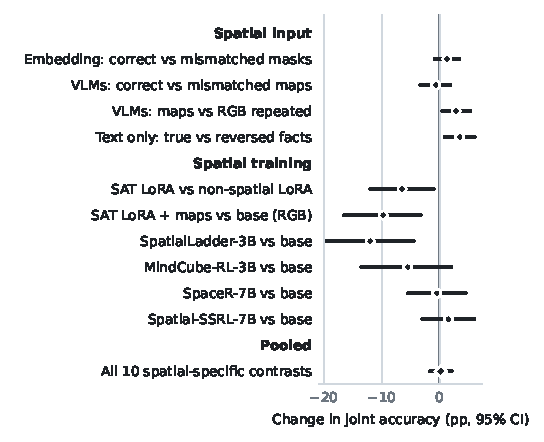
\includegraphics[width=\columnwidth]{forest_compact}
\caption{Change in EgoNormia joint accuracy (pp, 95\% CI). Spatial input: embedding with correct vs.\ mismatched masks; VLMs with correct vs.\ mismatched maps and with maps vs.\ RGB repeated; text-only true vs.\ reversed facts. Spatial training: SAT LoRA vs.\ non-spatial LoRA; SAT LoRA with maps vs.\ base on RGB; SpatialLadder-3B, MindCube-RL-3B, SpaceR-7B and Spatial-SSRL-7B vs.\ their bases. Diamond: pooled spatial-specific effect over ten contrasts.}
\label{fig:forest}
\end{figure}

\paragraph{Spatial input.}
The combined embedding makes geometry more readable (probe C5 $-$ C2 $+3.4\ [+2.2,+4.7]$; facing $+7.6$, hands $+4.3$) and gives a small social gain over C2 ($+2.6\ [+0.4,+4.9]$) but not over mismatched masks ($+1.3\ [-0.9,+3.4]$): extra input helps, correct geometry does not. Direct answering agrees: maps raise all three models over RGB by 4--6 pp (e.g., GPT-5.6 68.5$\to$74.5\%), yet mismatched maps do as well ($-0.7\ [-3.2,+1.8]$ pooled), spatial chain-of-thought is no better than generic (GPT-5.6 $-2.5$, Qwen3-VL-32B $-4.0$), and items rated as high spatial need gain no more than the rest ($-1.4\ [-4.6,+1.9]$). Spatial facts matter only without the image: reversing them in text-only descriptions costs $3.5$ pp pooled (Qwen3-VL-32B $5.5\ [+1.0,+10.6]$).

\paragraph{Spatial training.}
The SAT LoRA learns spatial QA (held-out SAT 88.8 vs.\ 78.8\%) but loses $6.5$ pp on EgoNormia against the control LoRA. Published fine-tunes agree: SpatialLadder-3B $-12.0\ [-19.5,-4.5]$ (its paper reports $+23.5$ on spatial benchmarks), MindCube-RL-3B $-5.5$, SpaceR-7B $-0.5$, Spatial-SSRL-7B $+1.5$; larger claimed spatial gains go with larger social costs (a trend over four models). With the full combined input (RGB, three maps, four descriptions) the SAT LoRA trails base Qwen3-VL-8B on RGB by $9.8$ pp; LoRA ($-5.0$, $p{=}.033$) and input ($-4.5$, $p{=}.16$) costs add without interaction ($-0.2$): the fine-tuned model does not learn to use the maps.

\paragraph{Failure analysis.}
Most between-condition differences are abstention. EgoNormia's non-spatial scene description costs GPT-5.6 $9$ pp, entirely through extra ``None'' picks (13$\to$38), and a mismatched scene description costs Qwen3-VL-32B $22$ pp: models follow wrong text while ignoring wrong maps. With ``None'' removed, conditions converge (GPT-5.6 71.5--73.0\%, Qwen3-VL-32B 67.0--70.0\%), and Gemini~4's gain from maps is fewer ``None'' picks (40$\to$27) at flat conditional accuracy. A GPT-5.6 judge labelled each wrong answer: about one in 63--87 per model is spatial, about 60\% are perception errors (who is present, attending or gesturing) and 20--31\% are norm errors; a Gemini~4 second rater ($\kappa{=}.35$) agrees that spatial errors are rare.

\paragraph{Cross-model evidence.}
Across 30 models with published spatial and social-reasoning scores, the two correlate (composite Spearman $+0.69$, $p{<}.001$) but only at $+0.15$ ($p{=}.50$) after controlling for MMMU. Within one evaluator (OpenCompass, 284 models), MMBench Social Relation tracks Spatial Relationship ($+0.62\to+0.25$ partial) no more closely than OCR ($+0.63\to+0.31$) or celebrity recognition ($+0.59\to+0.36$) (Figure~\ref{fig:litscaling}). This observational evidence points to general capability rather than a specific spatial--social link, consistent with our interventions; no prior work we found tests the transfer directly.

\begin{figure}[t]
\centering
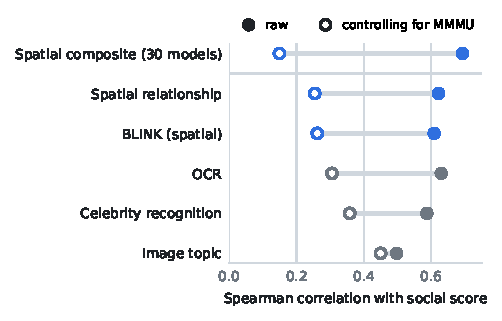
\includegraphics[width=\columnwidth]{lit_compact}
\caption{Spearman correlation with social score, raw (filled) vs.\ controlling for MMMU (open). Top row: spatial composite across 30 models. Remaining rows: MMBench Social Relation vs.\ spatial relationship, BLINK, OCR, celebrity recognition and image topic (284 models, one evaluator).}
\label{fig:litscaling}
\end{figure}

\paragraph{Limitations.}
With $n{=}200$, effects below about 3 pp cannot be excluded; the probe labels share extractors with the maps; and API results are single runs (GPT-5.6 agrees with itself on 83--90\% of items).

\subsection{Updated Research Idea}
\label{sec:idea5-updated}

\paragraph{Claim.}
Our results support a stronger statement than the proposal set out to test: improving a vision--language model's spatial ability does not improve, and may harm, its social-norm reasoning. Four lines of evidence agree (spatial-specific pool $+0.2\ [-1.7,+2.1]$; SAT LoRA $-6.5$ against a matched control; larger claimed spatial gains with larger social costs across four published fine-tunes; cross-model co-variation explained by general ability), but each rests on one benchmark, one training set and two model families. We therefore replace the plan to exploit spatial or pose signals with a study designed to establish, or overturn, the claim regardless of model, architecture, training data or evaluation set.

\paragraph{Factorial design.}
We cross four factors: \emph{scale} (about 1B to 72B within a family); \emph{family} (Qwen-VL, InternVL, LLaVA-OneVision, Gemma); \emph{spatial data}, namely static single-image QA (SAT), synthetic 3D and multi-view scenes, real-world depth and distance QA, egocentric video spatial QA, and body/pose-centric QA in which per-person keypoints and orientation from a human-centric encoder (e.g., Meta's Sapiens2) are rendered into the image and queried in text, so pose reaches both the visual and the language stream and a null cannot be blamed on how pose was fed in; and \emph{method} (LoRA, full fine-tuning, published checkpoints against their bases). Every spatial run is paired with a non-spatial control fine-tune of identical recipe, data size and token budget, as the SAT/VQAv2 pair was, and the quantity of interest is always the spatial-specific difference $\delta$.

\paragraph{Manipulation check.}
A run enters the analysis only if it improves held-out spatial benchmarks (VSI-Bench, MMSI-Bench, BLINK spatial); its spatial gain $g$ is the mean improvement over its control in pp, so the grid spans a range of doses.

\paragraph{Social evaluation.}
EgoNormia is joined by SIV-Bench, MuMA-ToM and MMToM-QA, EmoBench-M and Social-IQ~2.0 (norms, theory of mind, emotion and interaction in images and video), each scored under forced choice as well as its native format to remove the abstention confound that drove most condition effects above.

\paragraph{Statistics.}
A null claim needs an equivalence test, not a failed significance test. For each model--data--evaluation cell we pre-register a smallest effect of interest $\Delta=2$ pp and test
\begin{equation}
H_0:\ |\delta|\ge\Delta\quad\text{against}\quad H_1:\ |\delta|<\Delta,
\end{equation}
rejecting $H_0$ when the 90\% confidence interval of $\delta$ lies within $(-\Delta,\Delta)$ (two one-sided tests). A power analysis fixes items and seeds per cell, since our $n{=}200$ cells cannot exclude effects below about 3 pp. Across cells, a mixed-effects dose--response model with random effects for model $m$, data type $d$ and evaluation set $e$,
\begin{equation}
\delta_{m,d,e}=\beta_0+\beta_1 g_{m,d}+u_m+v_d+w_e+\varepsilon_{m,d,e},
\end{equation}
asks whether larger spatial gains buy larger social gains; the claim holds if the upper confidence bound of $\beta_1$ is at or below zero (or a small pre-registered bound) and $\beta_0$ is equivalent to zero.

\paragraph{Falsification.}
The claim is overturned if any cell with a verified spatial gain shows a spatial-specific social improvement whose lower 90\% confidence bound exceeds $\Delta$, replicated across seeds and at least two evaluation sets, or if the lower bound of $\beta_1$ is positive.
